\documentclass[conference]{IEEEtran}

\usepackage[T1]{fontenc}
\usepackage[utf8]{inputenc}
\usepackage{cite}
\usepackage{amsmath,amssymb}
\usepackage{graphicx}
\usepackage{booktabs}
\usepackage{xcolor}
\usepackage{hyperref}
\usepackage{microtype}
\usepackage{pifont}

\hypersetup{hidelinks}

\newcommand{\cmark}{\ding{51}}
\newcommand{\xmark}{\ding{55}}

% Correct bad hyphenation
\hyphenation{CultiVar}

% ============================================================
\begin{document}

\title{CultiVar-17: One-Shot Digit Recognition with a\\
       Culturally-Motivated Style Taxonomy}

\author{%
  \IEEEauthorblockN{Attila Torda}
  \IEEEauthorblockA{%
    DigitRecognizer Project\\
    \textit{[affiliation placeholder]}
  }
}

\maketitle

% ============================================================
\begin{abstract}
We introduce CultiVar-17, a compact dataset of 17 hand-drawn digit templates that captures
stylistic variation motivated by regional and educational handwriting conventions—crossed
vs.\ uncrossed zero, European vs.\ American seven, serif vs.\ plain one, and more.
Using only these 17 templates as supervision, we train a CNN and a prototype-embedding model
via synthetic augmentation and evaluate transfer to the MNIST test set.
Our best configuration—a prototype-embedding model with full augmentation—achieves
$77.46 \pm 2.39\%$ MNIST accuracy from 17 examples, reaching 78\% of supervised CNN
performance.
An ablation study shows that elastic distortion and stroke-width perturbation contribute
independently and additively.
All code and data are publicly available for reproducibility.
\end{abstract}

\begin{IEEEkeywords}
one-shot learning, digit recognition, handwriting style, data augmentation, prototype
networks, MNIST
\end{IEEEkeywords}

% ============================================================
\section{Introduction}

Learning from very few examples is a longstanding challenge in machine learning
\cite{Koch2015,Vinyals2016,Snell2017}.
Handwritten digit recognition has served as a foundational benchmark since LeCun
et~al.\ \cite{LeCun1998} established MNIST, yet standard pipelines assume thousands of
labelled samples per digit class.

This work explores a strict one-shot regime: we build a complete recognition pipeline from
exactly \textbf{one hand-drawn template per class}, structured around a culturally-aware
17-class taxonomy.
Our contributions are threefold:

\begin{enumerate}
  \item \textbf{CultiVar-17}—a 17-template dataset encoding documented regional writing
        variants, distributed as a reproducible \texttt{.npy} artifact.
  \item \textbf{A one-shot augmentation pipeline}—elastic distortion, stroke-width
        perturbation, and affine noise applied to templates, generating diverse training
        batches from a single source.
  \item \textbf{An empirical study}—comparing nearest-template, CNN, and
        prototype-embedding approaches with ablation over augmentation components,
        achieving $77.46\%$ MNIST accuracy from 17 examples.
\end{enumerate}

% ============================================================
\section{Related Work}

\subsection{One-Shot and Few-Shot Learning}

Koch et~al.\ \cite{Koch2015} proposed Siamese Networks for one-shot image recognition,
learning a similarity metric between pairs of examples.
Vinyals et~al.\ \cite{Vinyals2016} introduced Matching Networks, which use
attention-weighted nearest-neighbour classification in an embedding space conditioned on the
support set.
Snell et~al.\ \cite{Snell2017} proposed Prototypical Networks, classifying by computing
Euclidean distances to class prototype embeddings—the architecture we adopt here.
Finn et~al.\ \cite{Finn2017} introduced MAML, a gradient-based meta-learning approach that
learns an initialisation enabling fast adaptation with few gradient steps.

\subsection{Handwriting Datasets and Cultural Variation}

Lake et~al.\ \cite{Lake2015} introduced Omniglot, a 1{,}623-character handwriting dataset
covering 50 alphabets from diverse writing systems, which became the canonical few-shot
classification benchmark.
CultiVar-17 is complementary in scope: rather than cross-alphabet generalisation, it targets
intra-digit stylistic variation driven by documented regional conventions.
LeCun et~al.\ \cite{LeCun1998} established MNIST as the standard digit recognition
benchmark; we use MNIST as the transfer target throughout.

\subsection{Data Augmentation for Handwriting}

Simard et~al.\ \cite{Simard2003} demonstrated that elastic distortions—smooth random
displacement fields applied to handwritten characters—substantially improve CNN
generalisation on MNIST.
We apply the same elastic distortion technique as a core augmentation component, combined
with stroke-width perturbation.
Our ablation (Section~\ref{sec:ablation}) confirms their independent and additive
contributions.

% ============================================================
\section{CultiVar-17 Dataset}

\subsection{Cultural Motivation}

Handwriting style reflects regional education systems and typographic conventions.
We document seven split points in standard digit classes, shown in
Table~\ref{tab:variants}.
Digits 3, 5, 6, and 8 have no variant split, yielding $6 \times 2 + 1 \times 3 + 4 = 17$
classes in total.

\begin{table}[t]
  \caption{Cultural motivation for CultiVar-17 variant splits.}
  \label{tab:variants}
  \centering
  \begin{tabular}{@{}clll@{}}
    \toprule
    Digit & Var.\,A & Var.\,B & Driver \\
    \midrule
    0 & uncrossed   & crossed         & zero-slash convention \\
    1 & plain vert. & serif / angled  & American vs.\ European \\
    2 & looped base & angular base    & cursive vs.\ print \\
    4 & open top    & closed top (+ cursive) & printing vs.\ cursive \\
    7 & uncrossed   & crossed         & American vs.\ European \\
    9 & looped tail & straight tail   & print vs.\ cursive \\
    \bottomrule
  \end{tabular}
\end{table}

\subsection{Template Extraction}

Source: a single composite image generated with an AI image tool and manually verified
for legibility and distinctiveness.
Procedure: isolate the central strip; split into 17 equal horizontal slots;
foreground-tight crop and centre each digit onto a $28\times28$ canvas.
Figure~\ref{fig:templates} shows all 17 templates.

Output: \texttt{train\_images.npy} ($17\times28\times28$ uint8) and
\texttt{train\_labels17.npy} (labels 0--16).

\subsection{Class-to-Digit Mapping}

For MNIST evaluation, 17 style classes are collapsed to 10 canonical digits via a fixed
surjective map (\texttt{src/variants17/label\_schema.py}).
Each variant maps to its base digit (e.g., \texttt{0\_variant\_a} and
\texttt{0\_variant\_b} $\to$ 0).

% ============================================================
\section{Method}

\subsection{Augmentation Pipeline}

Given one template per class, we generate training batches via stochastic augmentation:

\begin{itemize}
  \item \textbf{Elastic distortion} \cite{Simard2003}: random displacement field
        ($\sigma\!=\!4$, $\alpha\!\in\![15,32]$), interpolated with Gaussian smoothing.
  \item \textbf{Stroke-width perturbation}: morphological dilation (\textit{disk\_dilate})
        or soft blur (\textit{blur\_soft}), radius~1.
  \item \textbf{Affine noise}: rotation $\pm8^\circ$, scale $\in[0.92, 1.08]$ per axis.
  \item \textbf{Additive noise}: Gaussian, std $\in[0.01, 0.03]$.
\end{itemize}

With 256 repeats per class, each epoch presents 4{,}352 synthetically varied examples.
Figure~\ref{fig:augmentation} illustrates the six augmentation modes.

\subsection{Models}

\textbf{CNN (SimpleCNN).}
Two convolutional blocks (conv $\to$ BN $\to$ ReLU $\to$ pool) followed by a
fully-connected head with 17-way softmax.

\textbf{Prototype embedding (EmbeddingCNN).}
The same convolutional backbone projects each image into a 64-dimensional embedding.
Prototypes are the mean embeddings of the 17 raw templates.
At test time a query is classified by nearest-prototype distance \cite{Snell2017}.

Both models use Adam ($\text{lr}=10^{-3}$, batch~128) for 8 epochs.

% ============================================================
\section{Experiments}

\subsection{Configurations}

Table~\ref{tab:configs} lists the five experimental configurations.
CNN configurations run for 3 seeds; the prototype model for 5 seeds.
Best-epoch MNIST accuracy is reported per seed.

\begin{table}[t]
  \caption{Experimental configurations.}
  \label{tab:configs}
  \centering
  \begin{tabular}{@{}lcc@{}}
    \toprule
    Config & Elastic prob & Stroke prob \\
    \midrule
    no\_aug\_cnn      & 0.00 & 0.00 \\
    elastic\_only\_cnn & 0.70 & 0.00 \\
    stroke\_only\_cnn  & 0.00 & 0.80 \\
    full\_aug\_cnn    & 0.70 & 0.80 \\
    proto (embedding) & 0.70 & 0.80 \\
    \bottomrule
  \end{tabular}
\end{table}

\subsection{Baseline}

\textbf{Nearest-template (L2)} \cite{Cover1967}: assign each MNIST image the digit label
of its closest template under Euclidean distance.
No training is required.

% ============================================================
\section{Results}

\subsection{Main Results}

Table~\ref{tab:main} reports MNIST test-set accuracy for all methods.
Figure~\ref{fig:results} visualises the comparison.

\begin{table}[t]
  \caption{MNIST test accuracy (mean $\pm$ std\,\%).}
  \label{tab:main}
  \centering
  \begin{tabular}{@{}lrc@{}}
    \toprule
    Method & Acc.\,(\%) & Seeds \\
    \midrule
    Nearest-template (L2)      & 38.60         & --- \\
    No-aug CNN                 & $51.20 \pm 1.86$ & 3 \\
    Full-aug CNN               & $65.19 \pm 2.14$ & 3 \\
    \textbf{Proto embedding}   & $\mathbf{77.46 \pm 2.39}$ & 5 \\
    \midrule
    Supervised CNN (reference) & 99.11         & --- \\
    \bottomrule
  \end{tabular}
\end{table}

The prototype-embedding model reaches $77.46\%$—\textbf{78\% of supervised CNN
performance}—from 17 templates.
Even the no-augmentation CNN ($51.20\%$) substantially outperforms the nearest-template
baseline ($38.60\%$), showing that training on augmented templates provides significant
discriminative capacity beyond simple template matching.

\subsection{Augmentation Ablation}
\label{sec:ablation}

Table~\ref{tab:ablation} reports the 2$\times$2 ablation of elastic distortion and
stroke-width perturbation.

\begin{table}[t]
  \caption{Augmentation ablation (CNN, 3 seeds, MNIST test \%).}
  \label{tab:ablation}
  \centering
  \begin{tabular}{@{}lccc@{}}
    \toprule
    Augmentation & Elastic & Stroke & Acc.\,(\%) \\
    \midrule
    None                   & \xmark & \xmark & $51.20 \pm 1.86$ \\
    Elastic only           & \cmark & \xmark & $56.79 \pm 4.44$ \\
    Stroke only            & \xmark & \cmark & $55.59 \pm 0.78$ \\
    Elastic + stroke (full)& \cmark & \cmark & $65.19 \pm 2.14$ \\
    \bottomrule
  \end{tabular}
\end{table}

Both components independently improve accuracy by $\sim\!5$ percentage points over no
augmentation, and their combination yields a further gain (${\sim}9$~pp over elastic alone).
The higher variance of \textit{elastic\_only} ($\pm4.44$) versus \textit{stroke\_only}
($\pm0.78$) suggests elastic distortion is more seed-sensitive, while stroke perturbation
provides more consistent improvement.

% ============================================================
\section{Discussion}

Three patterns emerge:

\textbf{Augmentation is essential.}
The gap between nearest-template ($38.60\%$) and full-aug CNN ($65.19\%$) confirms that
synthetic diversity substantially improves generalisation beyond direct pixel matching.

\textbf{Embedding beats classification.}
The prototype model ($77.46\%$) outperforms the classification CNN ($65.19\%$) despite using
the same backbone, consistent with findings from Snell et~al.\ \cite{Snell2017} that the
metric-learning objective is better matched to the few-shot regime.

\textbf{The ceiling is style coverage, not capacity.}
Even at $77.46\%$, the system falls 22~pp short of supervised accuracy.
This gap reflects the fact that 17 templates cannot cover all handwriting styles in MNIST
regardless of augmentation or model complexity.

% ============================================================
\section{Threats to Validity}

\begin{itemize}
  \item \textbf{Single-source template bias}: all 17 templates originate from one
        AI-generated composite image and reflect a single stylistic hand.
  \item \textbf{Limited augmentation family}: elastic and stroke perturbations may
        under-represent real handwriting variability (pen angle, slant, baseline drift).
  \item \textbf{Projection artefacts}: the 17$\to$10 class collapse may hide class-specific
        errors; a full 17-way confusion matrix would give a more complete picture.
\end{itemize}

% ============================================================
\section{Future Work}

Adding even 2--3 real handwriting samples per style cluster would substantially broaden
template coverage.
Stronger augmentation (local nonlinear warps, pen-angle simulation) and meta-learning
objectives such as MAML \cite{Finn2017} or Matching Networks \cite{Vinyals2016} could
further improve generalisation.
Extending CultiVar-17 to additional cultural conventions and non-Latin scripts is a natural
next step for the dataset contribution.

% ============================================================
\section{Reproducibility}

All experiments are reproducible with a single command:

\begin{verbatim}
python scripts/run_oneshot_experiment.py \
       --ablation --proto-seeds 5
\end{verbatim}

Figures are regenerated with:

\begin{verbatim}
python scripts/make_figures.py
\end{verbatim}

Raw results are stored in
\texttt{experiments/reports/oneshot\_results.json}.

% ============================================================
\section*{Acknowledgements}

[Acknowledgements placeholder.]

% ============================================================
\begin{figure}[t]
  \centering
  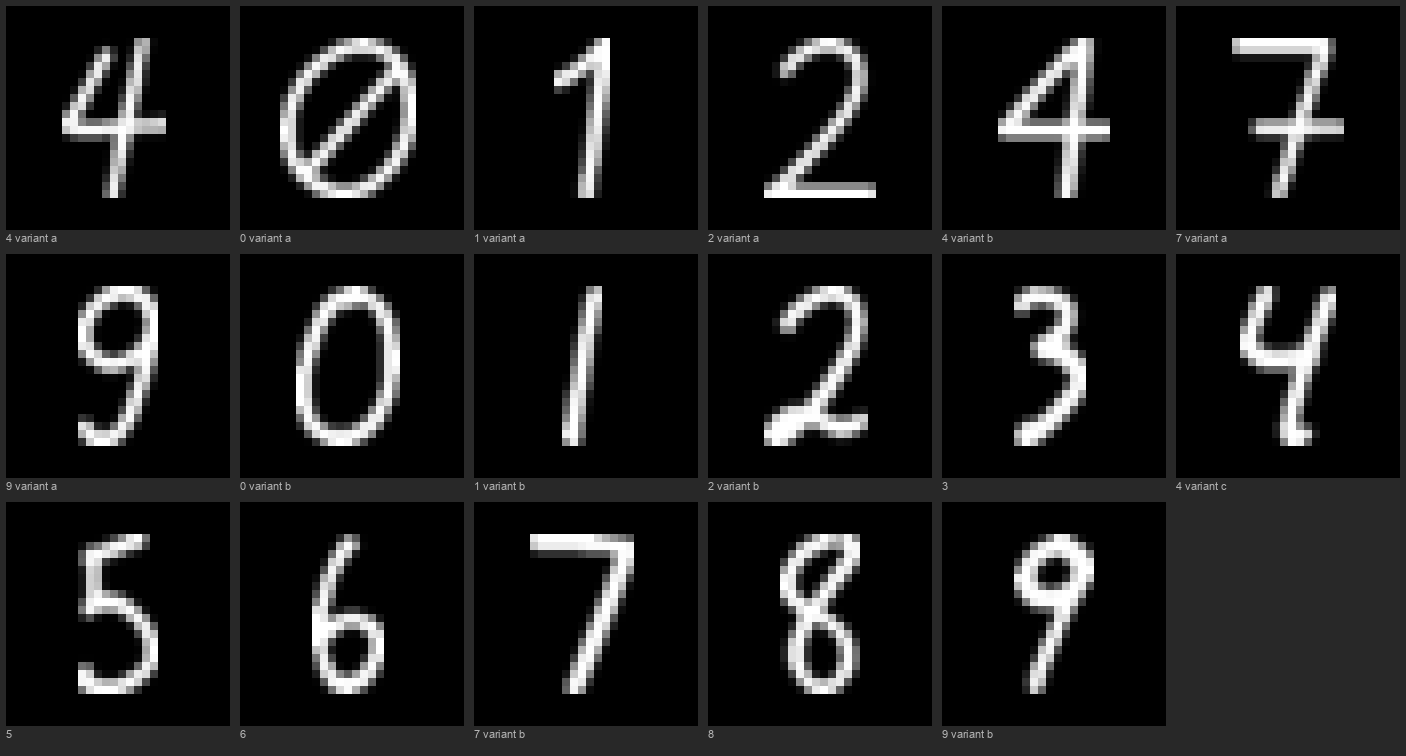
\includegraphics[width=\columnwidth]{figures/fig1_templates.png}
  \caption{All 17 CultiVar templates ($8\times$ upscaled). Class labels below each
           digit indicate the style variant.}
  \label{fig:templates}
\end{figure}

\begin{figure}[t]
  \centering
  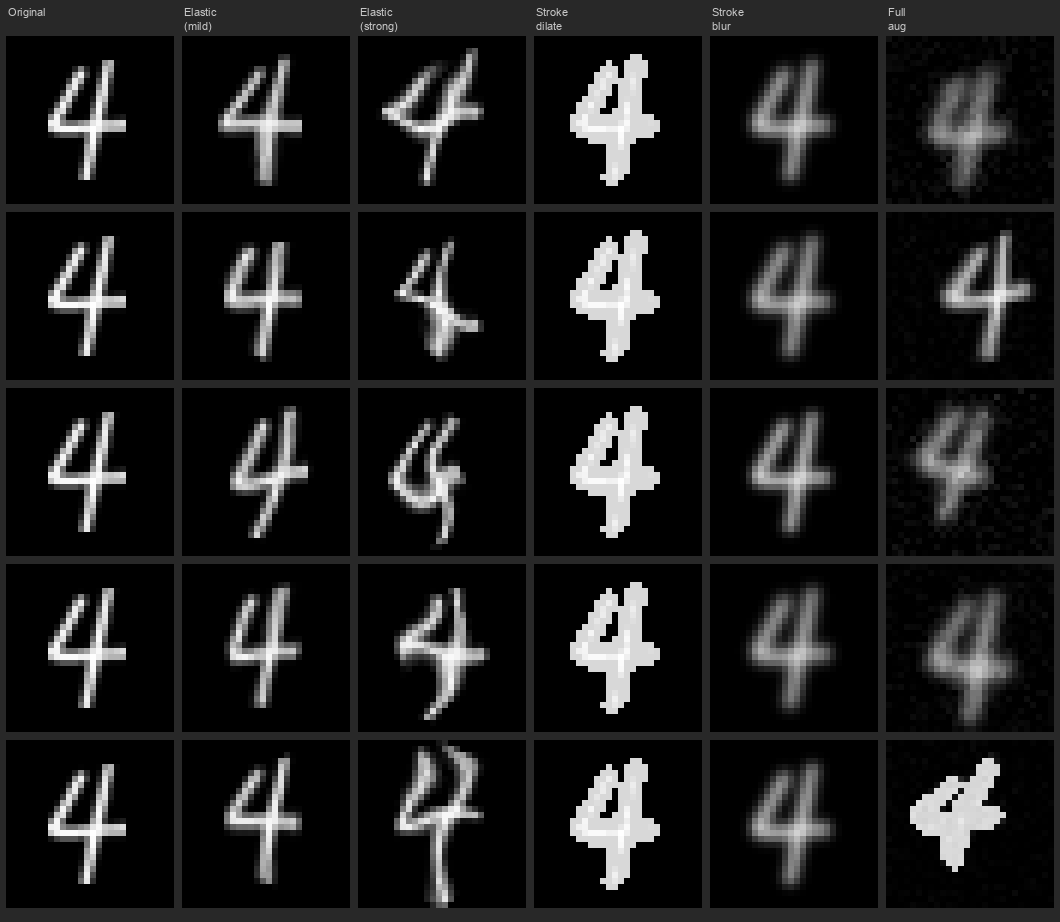
\includegraphics[width=\columnwidth]{figures/fig2_augmentation.png}
  \caption{Augmentation gallery for template~0 (\texttt{4\_variant\_a}). Columns left
           to right: original, elastic (mild), elastic (strong), stroke dilate, stroke
           blur, full augmentation (5 samples each).}
  \label{fig:augmentation}
\end{figure}

\begin{figure}[t]
  \centering
  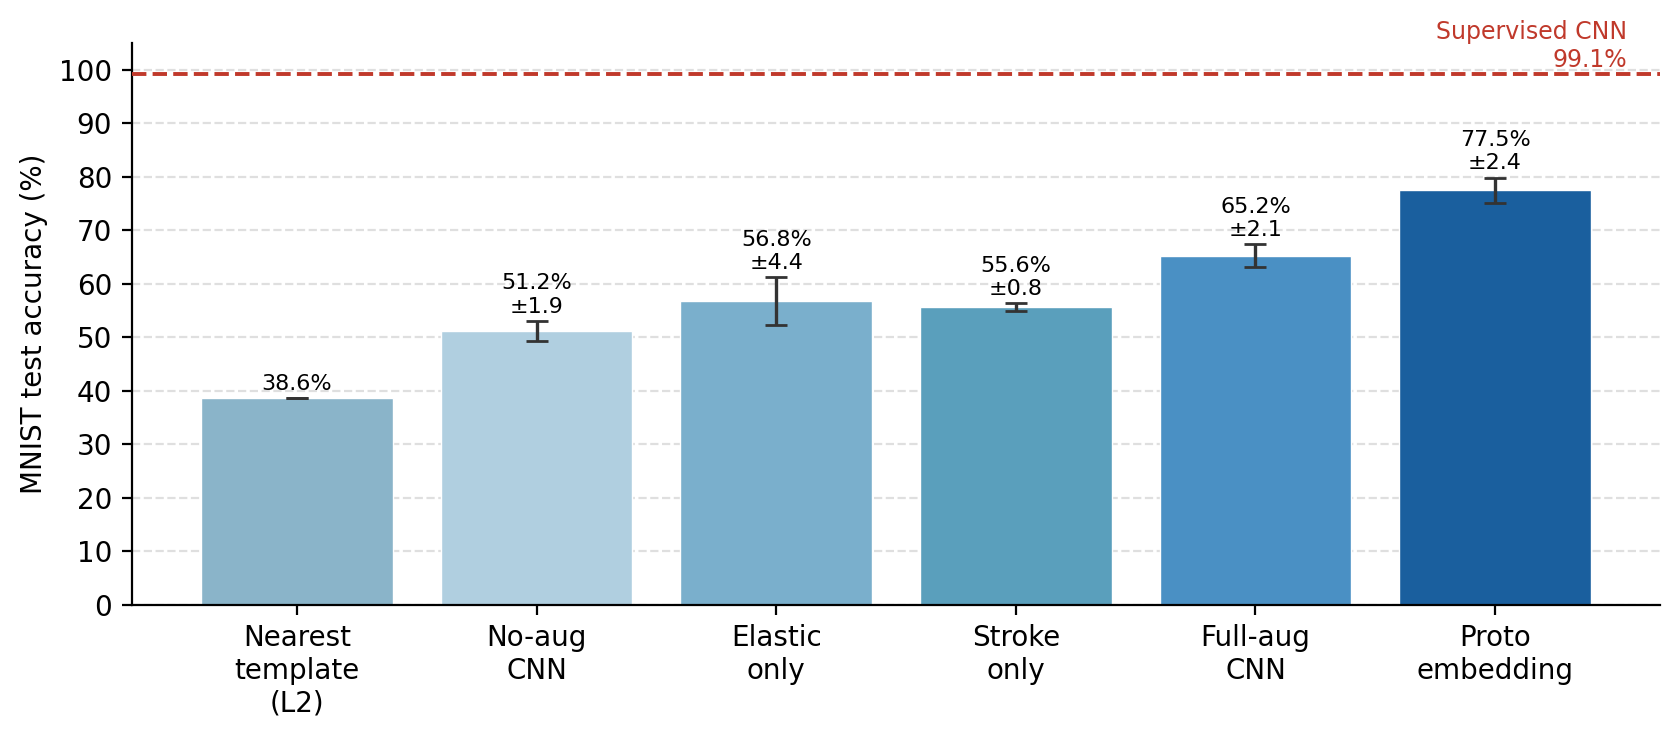
\includegraphics[width=\columnwidth]{figures/fig3_results.png}
  \caption{MNIST test accuracy for all one-shot configurations. Error bars show
           $\pm1$ standard deviation across seeds. Dashed line: supervised CNN reference
           ($99.11\%$).}
  \label{fig:results}
\end{figure}

% ============================================================
\bibliographystyle{IEEEtran}
\bibliography{cultivar17_refs}

\end{document}
